\chapter{ Marco temático: Producción de cerveza artesanal}
    
    \par Según definición del Código Alimentario Argentino (Ley 18284, 2017, art. 1080 y 1082 bis) “Cerveza es la bebida resultante de fermentar, mediante levadura cervecera, al mosto de cebada malteada sometido previamente a un proceso de cocción, adicionado de lúpulo...”. Este denomina, de “\textit{Elaboración Artesanal} a aquella cerveza que cumpla con las siguientes exigencias: a) Que no utilice en su producción aditivos alimentarios; y b) Que se encuentre adicionada únicamente con ingredientes naturales; y c) Que la elaboración sea de manera manual o semiautomática; y d) Que en el caso que se le agregue jugos o extractos de frutas, éstos sean previamente pasteurizados...”. 
    
    \par A continuación será desarrollado y explicado el proceso de fabricación de cerveza artesanal, con especial atención en el subproceso de maceración.
    
    \section{Insumos intervinientes}
        \par En la elaboración de cerveza se requieren cuatro ingredientes: cebada malteada, lúpulo, levadura y agua. El conocimiento de las propiedades de estas materias primas, su influencia sobre el proceso de elaboración y el producto final proporciona el fundamento para su tratamiento  y  procesamiento.
        
        
    	
        \subsection{Cebada: Grano y Malteado}
            \subsubsection{Grano: primeros procesos de su desarrollo}
                \par La cebada (\textit{Hordeum vulgare}) es un cereal que suministra el almidón necesario para la fabricación de cerveza, el cual es transformado posteriormente, en el proceso de cocción, en extracto fermentable.
                \par La estructura interna del grano se divide en tres partes principales: la \textit{región germinal}, que cuenta con el embrión, el \textit{endospermo}, compuesto por gránulos de almidón separados por una matriz de contenido proteico y envuelto por una capa llamada aleurona, y las \textit{cubiertas del grano}, las cuales son cáscaras compuestas de celulosa que recubren el grano (Véase Figura \ref{EstructuraGrano}).
        
                \par El almidón es el componente más importante de la cebada, el cual ocupa entre 50\% - 65\% de su composición. Los gránulos de almidón, denominados amiloplastos, se componen por dos estructuras diferentes: La Amilopectina (presentes entre un 75\% - 80\%) y la Amilosa (presentes entre un 20\% - 25\%), ambas formadas por residuos de glucosa con diferentes propiedades de degradación debido a sus correspondientes estructuras (con y sin ramificaciones, respectivamente). La capa que rodea a los gránulos de almidón se encuentra formada por $\beta$-glucano (presente entre un 80\%-90\%) y pentosano (presente en un 10\%-20\%).
        
                \begin{figure} [h]
		            \centerline{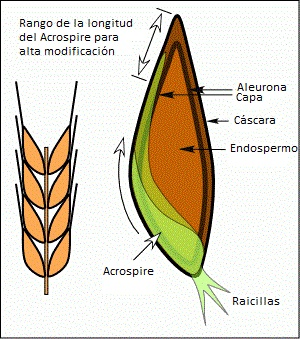
\includegraphics[scale=0.9]{estructura_de_grano.jpg}}
		            \caption{Esquema del grano de cebada}
	                \label{EstructuraGrano}
    	        \end{figure}
    	
    	        \paragraph{Germinación}
    	        Es el proceso de crecimiento del germen de cada semilla, el cual comienza en un ambiente con condiciones necesarias (agua, oxígeno, y temperatura apropiada). Durante este proceso se liberan las enzimas de la cubierta de aleuronas, y se crean otras nuevas que atraviesan la matriz de proteínas/carbohidratos de almidón del endosperma, dividiendo la misma en carbohidratos, aminoácidos y lípidos más pequeños que posibilitan el desarrollo de las reservas de almidón de las semillas.
    	
    	        \paragraph{Modificación}
    	        El grado en el cual las enzimas desgarran y abren esa capa, y comienzan a liberar los gránulos de almidón (es decir, rompen el endosperma), para ser usados en el crecimiento de la planta, es conocido como modificación. Un indicador visual para juzgar el grado de modificación es la longitud del acrospire que crece bajo el endosperma. El largo del acrospire en una malta altamente modificada típicamente será el 75\% - 100\% del largo de la semilla (Véase Figura \ref{EstructuraGrano}). 
    	    \subsubsection{Malteado}
    	        \par El malteado es el proceso por el cual los granos de cebada son remojados y escurridos para iniciar la germinación de la planta desde la semilla. Luego de un periodo determinado, los granos son secados en un horno (\textit{Kiln}) con el fin de detener las enzimas hasta que el fabricante los utilice.
    	        
    	        \par El propósito de maltear un grano es el de alcanzar el grado de modificación requerido para el proceso en el cual será utilizado.
    	   
        \subsection{Lúpulo}
            \par El lúpulo (\textit{Humulus lupulus  L.}) es una planta trepadora, perenne, dioica, perteneciente al grupo de las urticáceas y la familia cannabaceae. En la fabricación de cerveza, son utilizadas únicamente las inflorescencias de las plantas femeninas, estas contienen las resinas amargas y los aceites etéreos que le suministran a la cerveza amargor y componentes aromáticos (Kunze, 2006).
            
        \subsection{Levadura}
            \par La levadura es un hongo unicelular, el cual es capaz de cubrir su demanda de energía para sus funciones vitales en presencia de oxígeno (aerobio), por respiración, y en ausencia de oxígeno (anaerobio), por fermentación donde el azúcar es convertido a alcohol y dióxido de carbono.
            
            \par La levadura no realiza únicamente la fermentación alcohólica, sino que también tiene, debido a su metabolismo, una gran influencia sobre el sabor y el carácter de la cerveza.
            
            \par Existen dos variedades de levadura (\textit{Lager} o \textit{Ale}). Según cada una de estas, varía la duración y el rango de temperatura utilizados durante el proceso de fermentación.
            
        \subsection{Agua}
            \par Cuantitativamente, el agua es la materia prima más abundante en la cerveza (aproximadamente el 95\%). Su obtención y tratamiento es de particular importancia para el cervecero, dado que su composición (minerales presentes) influye sobre la conversión de almidones durante la maceración, la regulación del pH y acentuación de perfiles tanto a malta como a lúpulo. Además, la presencia de algunos minerales, como el calcio, garantizan la vitalidad del mosto para una fermentación saludable.
            
    \section{Resumen de proceso completo de fabricación de Cerveza Artesanal}
        \par El proceso de producción de cerveza artesanal se divide en 7 etapas consecutivas, resumidas a continuación:
        
        \begin{enumerate}
            \item \textit{Maceración}: Infusión de malta en agua a una temperatura específica según el tipo de macerado elegido. Produciendo, conforme la temperatura y pH del preparado, la activación (o desnaturalización) de enzimas con el propósito de degradar/convertir la proteína y los almidones en azúcares, aminoácidos y lípidos, entre otros subproductos. La solución de granos y agua producidos en esta etapa recibe el nombre de mosto.
            
            \par Este proceso es de particular importancia para asegurar las condiciones que afectan las actividades de alimentación y reproducción de la levadura en la etapa de fermentación, como son la cantidad de azúcares y proteínas del mosto.
            
            \item \textit{Recirculado}: Procedimiento en el cual se extrae el mosto del macerador libre de partes de grano o cáscaras. Este involucra un aumento de temperatura para mejorar la fluidez del líquido, un proceso de filtrado y, por último, un lavado de los granos para la extracción del azúcar remanente en las cáscaras.
            
            \item \textit{Cocción}: Etapa de eliminación de bacterias mediante pasteurización, floculación de proteínas, desnaturalización de enzimas y evaporación de elementos volátiles indeseados. Posee una duración variable y durante la misma son incorporados, en distintos momentos, los lúpulos de sabor y aroma.

            \item \textit{Enfriamiento}: Procedimiento en el cual el mosto es enfriado con celeridad a una temperatura de trabajo acorde a la cepa de levadura que se fuera a utilizar. La velocidad de enfriado permite mantener el mosto estéril y evitar la generación de sabores indeseados.

            \item \textit{Fermentación}: Etapa en la cual se incorpora levadura al mosto producido, para que a través de la inoculación de esta, se fermente el empaste y produzca así alcohol y otras características de la cerveza. 

            \item \textit{Maduración}: Estacionamiento de la cerveza en tanques a bajas temperaturas (0°C a -5°C) con el objetivo de acomodar los sabores de cada ingrediente, eliminar subproductos y clarificar por medio de filtrado por decantación.

            \item \textit{Filtrado}: Remoción de sedimentos excedentes del preparado. 
        \end{enumerate}
        
    \section{Maceración}
        \par La \textit{maceración} es un proceso de extracción y solubilización de sustancias que forman parte de la molienda. Esta última, se encuentra compuesta por elementos solubles (como azúcares, dextrinas y sustancias minerales) e insolubles (como el almidón y la celulosa de la cáscara, entre otras).
        
        \subsection{Las enzimas}
            \par Las enzimas son las encargadas de llevar a cabo la disociación de los sustratos insolubles, cuyas actividades dependen de un conjunto de factores, esencialmente, los valores de pH y temperatura del empaste. 
            % TODO poner la referencia a la tabla de enzimas.
            \par En la tabla \ref{tablaEnzimas} se detallan las principales enzimas intervinientes durante la maceración, su rango de temperatura de actividad, pH y función.
            \subsubsection{Actividades enzimáticas}
                \begin{enumerate}[a)]
                    \item \textit{Degradación del almidón}
                    % TODO poner la referencia a la tabla de enzimas.
                        \par La degradación del almidón, producido esencialmente por las enzimas $\alpha$ y $\beta$-amilasa (tabla \ref{tablaEnzimas}), produce azúcares a partir de las cadenas de dicha sustancia (Véase Figura \ref{DegradacionAlmidon}). Esta degradación ocurre en tres etapas consecutivas y bien diferenciadas (Kunze, 2006):
                        
                        \begin{enumerate}[1.]
                            \item Engrudamiento: Proceso de hinchamiento y reventamiento de los granos de almidón en solución caliente (60°C) y acuosa. Las moléculas de almidón liberadas en esta solución viscosa son mucho mejor atacadas por las amilasas que el almidón no engrudado.
                            
                            \item Licuefacción: Proceso de disminución de viscosidad del almidón por engrudado, por parte de la enzima $\alpha$-amilasa.
                            
                            \item Sacarificación: Proceso de degradación, por parte de las amilasas, del almidón licuado a maltosa y dextrinas límites.
                        \end{enumerate}
                        
                        \par Algunos de estos azúcares como la maltosa, la maltotriosa y la glucosa son más fácilmente procesados por la levadura y se los denomina \textit{azúcares fermentables}, mientras que los restantes reciben el nombre de \textit{azúcares no fermentables}, los cuales afectarán la densidad y el sabor final de la cerveza.
                        
                        \begin{figure}		                                                            \centerline{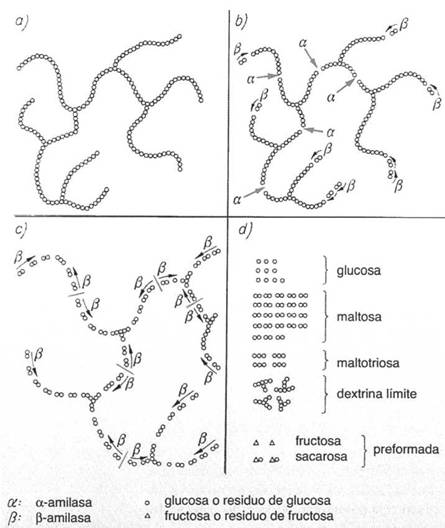
\includegraphics[scale=0.7]{degradacion_de_almidon.jpg}}
		                    \caption{Degradación cadena de almidón. a) Cadena de Almidón. b) Acción de $\alpha$-amilasa y $\beta$-amilasa. c) Aumento de acción $\beta$-amilasa y inactivación de $\alpha$-amilasa. d) azúcares obtenidos.}
	                        \label{DegradacionAlmidon}
    	                \end{figure}

                    \item \textit{Degradación del $\beta$-glucano}
                        \par El \textit{$\beta$-glucano} es una partícula de alto peso molecular cuya presencia enturbia la cerveza y produce la formación de geles, siendo esto último indeseado debido a las dificultades de filtración que acarrea. La molécula de $\beta$-glucano está formada por filamentos finos unidos por proteína, los cuales deben ser liberados para que sean solubles y así evitar las consecuencias antes mencionadas. La enzima \textit{$\beta$-glucanasa} libera los filamentos finos de su fijación de proteínas, la cual posee un rango de temperatura óptima de acción de 40-45 ºC. Además, la enzima \textit{$\beta$-glucanosolubilasa} actúa liberando proteínas que pueden ser consumidas por las levaduras posteriormente en el proceso de fermentación, siendo 62 ºC la temperatura óptima de actividad.
                        
                    \item \textit{Otros procesos de degradación}
                        \par Una parte de los fosfatos ligados de forma orgánica y aún no disueltos, es disuelta por las fosfatasas. Estos fosfatos son absolutamente necesarios para la realización de la fermentación alcohólica.
                        
                        \par Durante la maceración, con duración y temperaturas en aumento, son liberados taninos y antocianógenos de las cáscaras o del endospermo. Los taninos de alto peso molecular y los antocianógenos tienen una importancia esencial para la formación de turbidez en la cerveza, donde se combinan con substancias albuminoideas de alto peso molecular y precipitan. También tienen una influencia negativa sobre el sabor de la cerveza.
                \end{enumerate}
            \subsubsection{Influencia de factores externos}
                \par Los factores que influyen sobre la degradación son muy importantes para el cervecero, los de mayor influencia son:
                
                \begin{itemize}
                
                    \item {\textbf{Temperatura}:} Cada enzima tiene un rango de temperatura ideal de trabajo. Por debajo de este rango la actividad de la enzima disminuye, acorde se aumenta la temperatura se optimiza, en forma paulatina, su ciclo de acción hasta llegar al valor ideal de temperatura. Por encima de este rango la enzima se desnaturaliza por completo(Gráfica en Figura \ref{TemperaturaEnzimas})
                    
                    \begin{figure} [h]		                                                                \centerline{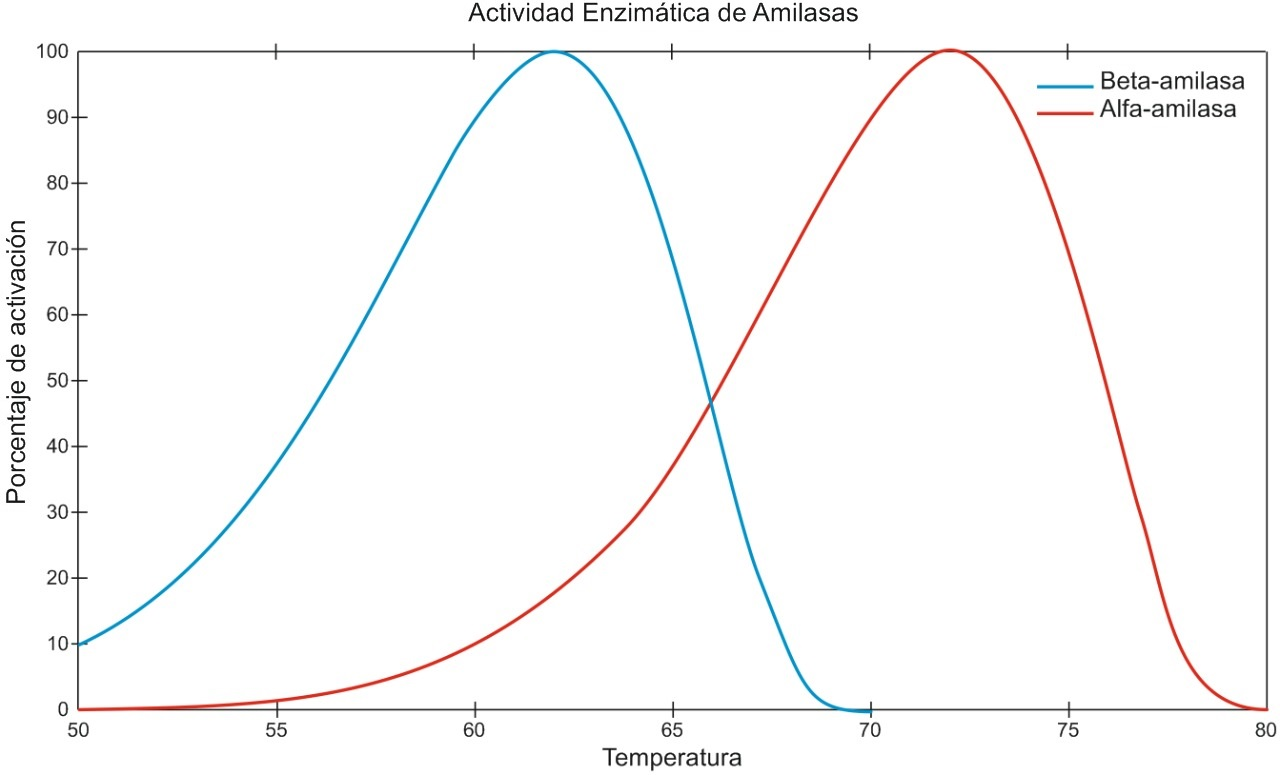
\includegraphics[scale=0.3]{temperatura_amilasas.jpg}}
		                \caption{Actividad enzimática respecto temperatura para enzima $\alpha$-Amilasa (Rojo) y $\beta$-Amilasa(Azul).}
	                    \label{TemperaturaEnzimas}
    	           \end{figure}
    	           
    	            \item {\textbf{La duración de la maceración}:} Las enzimas no actúan de forma uniforme durante el proceso de maceración(Véase Figura \ref{DuracionEnzimas}). Se pueden distinguir en la actividad de las enzimas dos etapas dependientes del tiempo:
    	            
    	                \begin{itemize}
    	                    \item El máximo de actividad enzimática es alcanzado entre los 10 a 20 minutos de comenzada la maceración.
    	                    
    	                    \item Luego, entre 40 y 60 minutos, la actividad disminuye primero de forma acelerada, decreciendo lentamente a continuación.
    	               
    	                \end{itemize}
    	                
    	                \begin{figure} [H]		                                                       \centerline{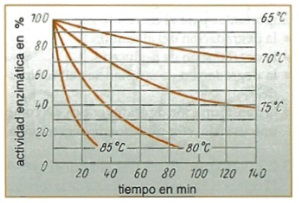
\includegraphics[scale=1.4]{duracion_amilasas.jpg}}
		                    \caption{Actividad enzimática respecto al tiempo a distintos niveles de temperatura.}
	                        \label{DuracionEnzimas}
    	                \end{figure}
    	                
    	           \item {\textbf{Influencia de pH}:} La actividad de las enzimas está ligada, también, al valor pH. Al igual que la temperatura, cada enzima, posee un rango de pH ideal para realizar su actividad (Véase Figura \ref{GraficoPhEnzimas}). Dentro del rango es posible incrementar el contenido de compuestos solubilizados, por el contrario, fuera del rango los valores de compuestos decrecen notablemente.
    	              
    	                \begin{figure} [H]		                                                       \centerline{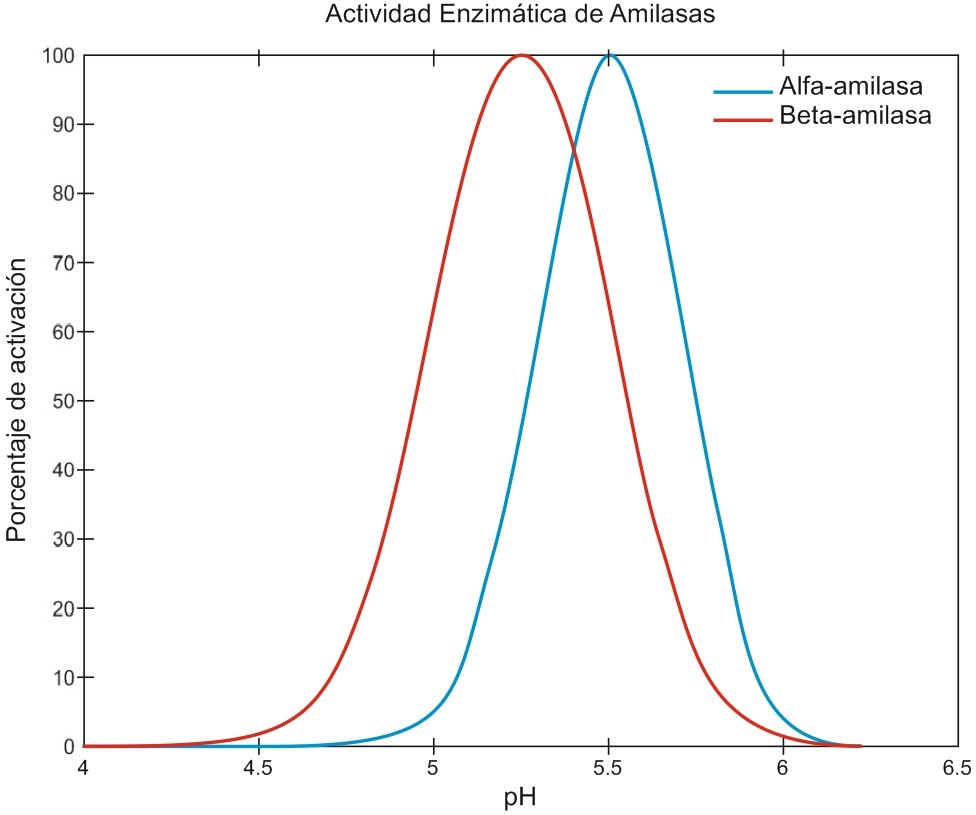
\includegraphics[scale=0.7]{activacion_pH.jpg}}
		                    \caption{Actividad enzimática respecto pH para enzimas $\alpha$-Amilasa (Azul) y $\beta$-Amilasa(Rojo).}
	                        \label{GraficoPhEnzimas}
    	                \end{figure}

                \end{itemize}
        \subsection{Composición del Extracto y Rendimiento del grano}
            \par Aproximadamente, del 75\% al 80\% de la masa de malta es disuelta durante la maceración, el residuo insoluble es separado con los desechos. Aproximadamente dos tercios del extracto formado durante la maceración (Ver imagen en Figura \ref{ComposicionExtracto}), 63 a 68\%, está compuesto por azúcares fermentables. La composición promedio de estos azúcares fermentables se pueden observar en la tabla \ref{tab:ComposicionAzucaresFermentables}.
            
            \begin{table}[h]
                \centering
                \begin{tabular}{|c|c|}
                    \hline
                     Azúcares fermentables &  Composición promedio \\
                     \hline
                     Maltosa & 65,5\% \\
                     \hline
                     Maltotriosa & 17,5\% \\
                     \hline
                     Sacarosa & 5\% \\
                     \hline
                     Glucosa y Fructosa & 12\% \\
                     \hline
                \end{tabular}
                \caption{Composición de azúcares fermentables}
                \label{tab:ComposicionAzucaresFermentables}
            \end{table}
            
            \par La parte restante, no fermentable del extracto, está compuesta principalmente por dextrinas límite, substancias albuminoideas (proteínas), gomas y minerales.
            \begin{figure} [H]		                                                                        \centerline{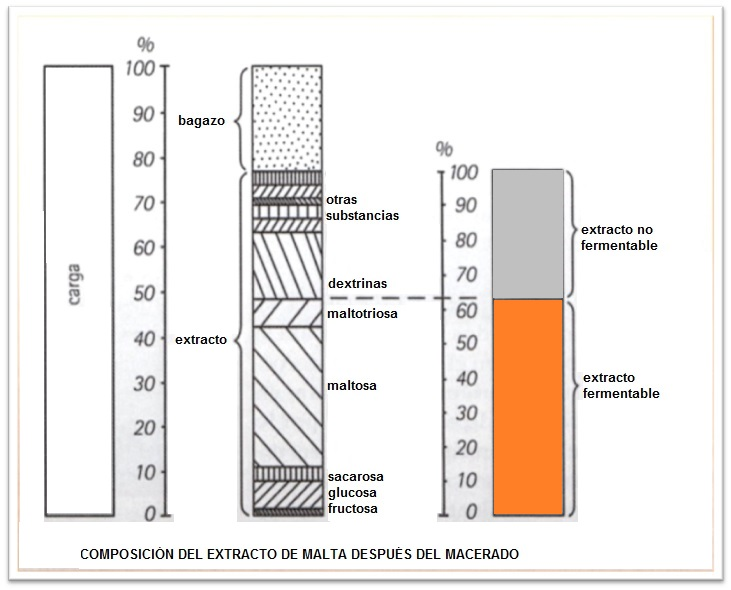
\includegraphics[scale=0.6]{composicion_luego_macerado.jpg}}
                \caption{Volumen inicial utilizado. Composición del extracto después del macerado. Rendimiento del grano.}
                \label{ComposicionExtracto}
            \end{figure}
            
            \par El porcentaje de la masa soluble del grano utilizada que realmente se disuelve en el líquido es conocida como rendimiento (Véase la tercer barra de la Figura \ref{ComposicionExtracto}). Un rendimiento con valor 100\% indica que en los desechos no hay presencia de sustancias solubles, es decir, hubo un máximo aprovechamiento de la materia prima. Cada tipo de grano posee tabulado el valor de rendimiento esperado, el cual es utilizado en los cálculos de planificación de la maceración. No obstante, este valor teórico puede variar según el procedimiento empleado y puede ser utilizado como criterio de evaluación del método que se lleva a cabo. La importancia del conocimiento de este valor radica en la relación directa que posee con la densidad obtenida luego de la maceración, la cual es determinante para las características de la cerveza buscada. 
            
        \subsection{Tipos de Maceración}
            \par Existen dos esquemas básicos de maceración: \textit{Infusión simple} y \textit{Maceración compleja}, diferenciados por la cantidad de saltos de temperatura ascendentes utilizados durante el proceso, y en forma adicional, el método por el cual son llevados a cabo estos cambios de temperatura.
            
            \begin{figure} [H]		                                                                    \centerline{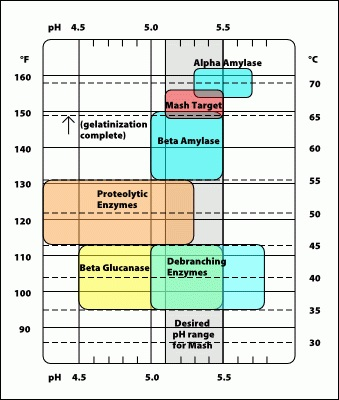
\includegraphics[scale=1]{activacion_enzimas_t_ph.jpg}}
                \caption{Rangos óptimos de temperatura y pH de activación de enzimas.}
                \label{ActivacionEnzimasTpH}
            \end{figure}
            
            \subsubsection{Proceso de maceración por Infusión}
                \begin{itemize}
                    \item \textbf{Infusión Simple}: Este proceso es utilizado en la mayor parte de los estilos de cerveza. Consiste en un sustento del empaste a una determinada temperatura constante, activando las enzimas amilasas durante todo el proceso. Para este tipo de maceración deben ser utilizadas maltas con alta modificación y poco contenido de $\beta$-glucano (cáscaras delgadas).
                    
                    \par El extracto obtenido por este proceso nunca es óptimo ya que es utilizada una temperatura promedio para activar ambas amilasas (Ver Figura \ref{TemperaturaEnzimas}), pero ninguna en particular de manera óptima.
                    
                    \par Ejemplo de procedimiento: \\ Se mezcla (infusiona) la malta molida con agua caliente para lograr una temperatura del empaste de 65,5ºC - 70ºC y un pH de 5,4 - 5,5 (Ver Figura \ref{ActivacionEnzimasTpH}). La mezcla debe ser mantenida a la temperatura de sacarificación durante un tiempo determinado (Ver Figura \ref{MaceracionSimple}).
                    
                    \begin{figure} [H]		                                                            \centerline{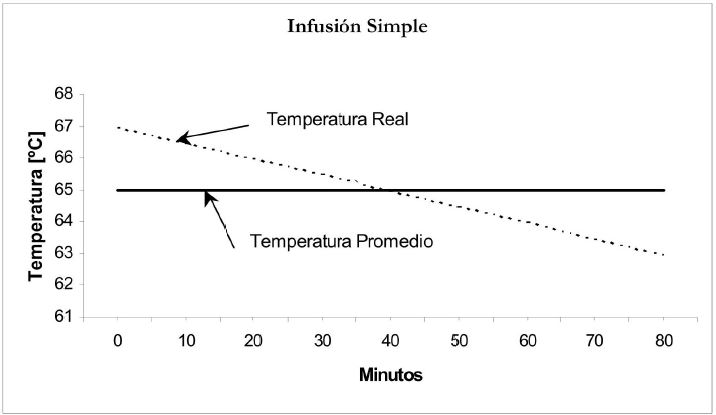
\includegraphics[scale=0.7]{maceracion_simple.jpg}}
                        \caption{Evolución temporal de temperatura en Maceración Simple}
                        \label{MaceracionSimple}
                    \end{figure}
                    
                    \item \textbf{Infusión Compleja (Maceración Escalonada)}: En la maceración compleja son utilizadas dos o más temperaturas para favorecer a diferentes grupos de enzimas. Esta consiste en realizar escalones de temperatura por cada enzima trabajada, desde las inferiores hasta las superiores. De esta manera, se logra una mayor obtención de extracto de la malta ya que se optimiza la activación de enzimas por medio de la temperatura (Ver Figura \ref{MaceracionEscalonada}).
                    
                    \par Este esquema es frecuentemente utilizado, y en algunos casos requerido, al incorporar ingredientes como arroz, maíz, cebada sin maltear, entre otros. Realizar este tipo de esquemas brinda en forma adicional diferentes aromas y sabores.
                    
                    \par Ejemplo de procedimiento: \\ Al comienzo se realiza una infusión simple, a temperatura de 50 °C óptima para la acción de las enzimas proteasas, $\beta$-glucanasas y peptidasa. Posteriormente, se aumenta un escalón de temperatura para mayor actividad de $\beta$-amilasa (60°C). Finalmente, se procede con un último escalón a 71°C de manera de aumentar el desempeño de la enzima $\alpha$-amilasa.
                    
                    \par Los valores de pH se mantienen dentro del rango 5,4 - 5,5. Si se calienta el macerador por calor directo este no se modifica, al contrario de cuanto se utiliza agregado de agua caliente, ya que la misma es más alcalina que el empaste.
                    
                    \begin{figure} [H]		                                                            \centerline{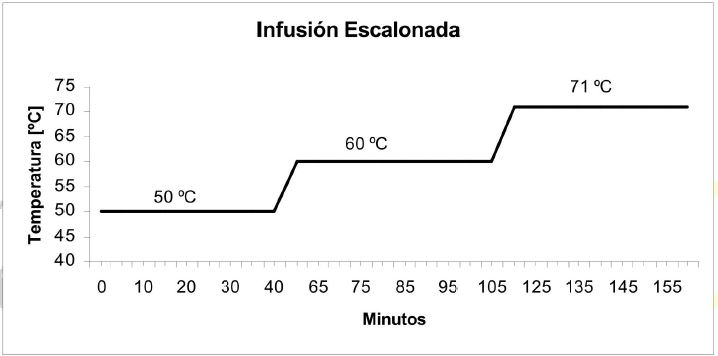
\includegraphics[scale=0.7]{maceracion_escalonada.jpg}}
                        \caption{Evolución temporal de temperatura en Maceración Escalonada}
                        \label{MaceracionEscalonada}
                    \end{figure}
                    
                \end{itemize}
                
            \subsubsection{Proceso de maceración por Decocción}
                \par En los procesos por decocción se extrae una parte del empaste, se la cuece y se lo reincorpora al resto aumentando la temperatura promedio total. Según la cantidad de cocciones de extracciones se distingue entre procesos de una, dos y tres decocciones.
            
                \par Los valores de temperatura y duración de cada cocción o escalón, difieren según el tipo de decocción. Respecto del pH, este es mantenido en el rango 5,4 - 5,5, siendo un valor común y óptimo para las enzimas involucradas.
                
                \par La extracción y cocción de templas hervidas tiene los siguientes efectos:
                
                \begin{itemize}
                    \item Una menor degradación de proteínas en la templa parcial, debido al calentamiento más rápido.
                    
                    \item Un control más enfocado de la actividad enzimática mediante el manejo de la temperatura y el tiempo, optimizando acción, y resultados de las actividades enzimáticas involucradas.
                    
                    \item Un engrudamiento y una licuación más extensiva del almidón, produciendo un mayor grado de extracción en las maltas.
                    
                    \item Un enjuague más intensivo de los componentes de las cáscaras.
                    
                    \item Una reducción de la cantidad de enzimas en la templa total.
                \end{itemize}
                
                \paragraph{Procesos de Decocción} A continuación se detallan procedimientos mas comunes de procesos de maceración por decocción simple, doble y triple.
                
                \begin{itemize}
                    \item \textit{Decocción Simple} \\ El sistema de decocción simple involucra un solo paso de decocción para obtener un escalón de proteasas y otro de degradación de almidón en azúcares. (Ver Figura 10).
                    
                        \begin{figure} [H]                      \centerline{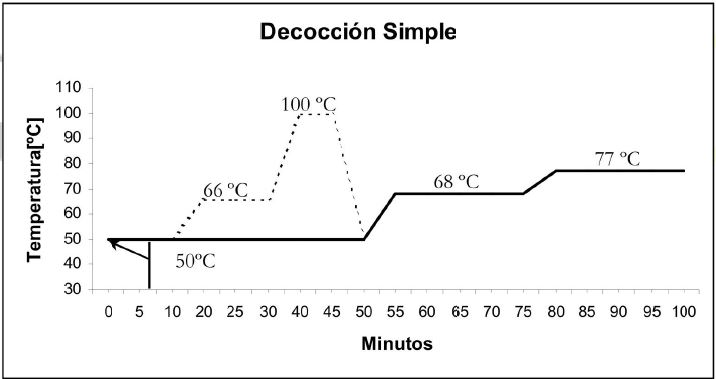
\includegraphics[scale=0.7]{decoccion_simple.jpg}}
                        \caption{Evolución temporal de temperatura en Maceración por Decocción Simple}
                        \label{MaceracionDecoccionSimple}
                    \end{figure}
                    
                    \item \textit{Decocción Doble} \\ La decocción doble incluye dos pasos de decocción para lograr la activación escalonada de proteasas, $\beta$-Amilasa y $\alpha$-Amilasa, (Ver Figura 11).
                    
                        \begin{figure} [H]		                                                            \centerline{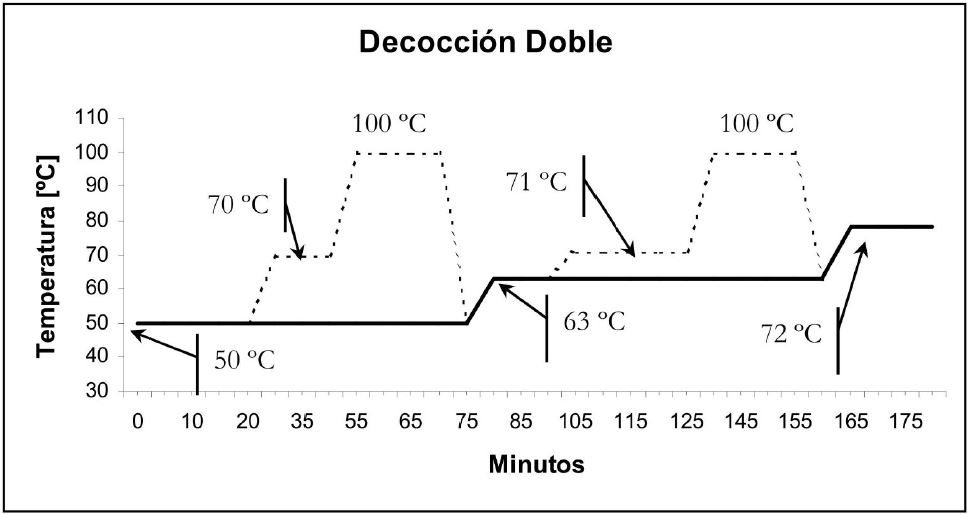
\includegraphics[scale=0.5]{decoccion_doble.jpg}}
                        \caption{Evolución temporal de temperatura en Maceración por Decocción Doble}
                        \label{MaceracionDecoccionDoble}
                        \end{figure}
                    
                    \item \textit{Decocción Triple} \\ La decocción triple involucra tres pasos de decocción para obtener cuatro escalones de activación de enzimas: $\beta$-glucanas, proteasas, $\beta$-amilasas, $\alpha$-amilasas, (Ver Figura 12).
                    
                        \begin{figure} [H]		                                                            \centerline{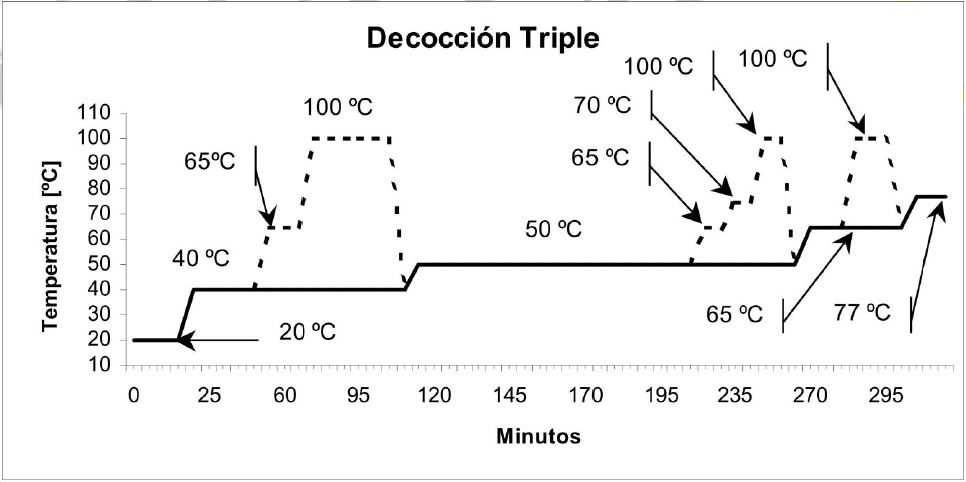
\includegraphics[scale=0.5]{decoccion_triple.jpg}}
                        \caption{Evolución temporal de temperatura en Maceración por Decocción Triple}
                        \label{MaceracionDecoccionTriple}
                        \end{figure}
                    
                \end{itemize}
        \subsection{Ecuaciones y procedimientos}
            \par Las variables que revisten interés al momento de planificar la maceración requieren de ciertos cálculos que serán enunciados en las siguientes subsecciones. 
            
            \subsubsection{Cálculo de rendimiento }
                \par Para determinar cuál fue el rendimiento obtenido en la maceración se debe conocer qué porcentaje del grano utilizado persiste en el mosto.
                
                Para saber la cantidad de extracto solubilizado en un litro de mosto luego de la maceración, se parte de:
                    
                    \begin{equation}
                        KgExt_{litro} = \frac{(DE-1) \cdot DE}{0.4}
                    \end{equation}
                    donde $DE$ es la densidad específica obtenida. Esta fórmula esta basada en los grados plato °$P$, que indican el porcentaje de extracto de malta sobre el peso del agua.
                    
                    \par Teniendo en conocimiento este valor, se debe ajustar al volumen de maceración con el que se trabaja, por tanto:
                    
                    \begin{equation}
                        KgExt_{total} = V \cdot KgExt_{litro}
                        \label{EcuacionExtractoTotal}
                    \end{equation}
                
                Entonces, el rendimiento de la maceración es:
                \begin{equation}
                    R_m = \frac{KgExt_{total}}{G}
                    \label{EcuacionRendimientoMaceracion}
                \end{equation}
                
                \par donde $R_m$ es el rendimiento de la maceración, $KgExt_{total}$ es la cantidad de extracto en el mosto y $G$ es la cantidad total de grano utilizado.
                
                \par Para obtener el rendimiento del equipo se promedia todos los valores obtenidos de cada maceración.
    
            
            \subsubsection{Cantidad de grano}
                \par Para determinar las cantidades necesarias de estas variables, el productor debe definir cuál es el volumen de producción deseado y la densidad que desea obtener.
                
                \begin{itemize}
                    \item \textbf{Cálculo de grano basado en el extracto potencial}
                    \par En este método de cálculo propuesto por Ray Daniels, se calcula la cantidad de cada tipo de grano involucrado en la receta, a partir del porcentaje utilizado según la misma y el extracto potencial de cada uno. 
                    
                        \par El \textit{extracto potencial} o \textit{poder diastácico} del grano es la proporción del mismo que puede solubilizarse. Este valor es calculado por el fabricante basado en experimentos realizados con el grano. A continuación se detallan algunos ejemplos: 
                        % TODO Agregar tabla con extractos potenciales de granos
                        \begin{table}[H]
                            \centering
                            \begin{tabular}{| c | c | c |}
                                \hline
                                Malta & Extracto Potencial & gr. Extracto / Kg. Grano \\
                                \hline
                                \hline
                                Pilsen & 81\% & 810
                                \\\hline
                                Caramelo & 73\%  & 730
                                \\\hline
                                Chocolate & 62\% & 620
                                \\\hline
                                Black Patent & 58\% & 580
                                \\\hline
                            \end{tabular}
                            \caption{Ejemplos de maltas con su correspondiente extracto potencial}
                            \label{tab:TablaExtractoPotencial}
                        \end{table}
                        
                        \par Para expresar la cantidad real de azúcares solubilizados en el volumen deseado, se utilizan los \textit{puntos de densidad (PD)}, que se calcula de la siguiente forma:
                        
                        \begin{equation}
                            PD = FD \cdot V
                        \end{equation}
                        donde $FD = (Densidad -1)\cdot 1000 $ es el \textit{factor denso} y $V$ es el volumen de mosto.
                        
                        \par Luego, para saber el aporte de azúcar $A_i$ que tiene cada grano se calcula:
                        
                        \begin{equation}
                            A_{i} = 8.316 \cdot 46 \cdot Ext_{i}                           
                        \end{equation}
                        donde \textit{8.316} es un factor de conversión de libra sobre galón (\textit{PPG, pounds per galon}) a kg sobre litro, \textit{46} es el valor máximo que se puede obtener (azúcar blanca que posee 100\% de extracto potencial) y $Ext_i$ es el extracto potencial del i-ésimo grano expresado en porcentaje.
                        
                        \par Por último, para saber la cantidad de kilogramos $G_i$ del i-ésimo grano que hay que utilizar, se emplea la fórmula:
                        
                        \begin{equation}
                            G_{i} = \frac{PD \cdot P_{i}}{A_{i} \cdot R_E} 
                            \label{EcuacionRayDaniels}
                        \end{equation}
                        donde $P_i$ es el porcentaje de utilización según la receta del i-ésimo grano y $R_E$ es el rendimiento del equipo, siendo utilizado el valor $0.7$ en una primera aproximación y luego ajustado a partir de los experimentos realizados.
                        
                    \item \textbf{Cálculo empírico basado en extracto obtenido} 
                    \par Para este cálculo, se debe conocer valores de densidad específica obtenidos en experimentos anteriores para estimar la cantidad de cada grano que hay que utilizar.
                    
                    \par Partiendo de la ecuación \ref{EcuacionRendimientoMaceracion}, para conocer la cantidad del i-ésimo grano a utilizar según el porcentaje del mismo en la receta será:
                    
                    \begin{equation}
                        G_{i} = \frac{KgExt_{total} * P_{i}}{R_E}
                        \label{EcuacionCantidadGranoEmpirico}
                    \end{equation}
                    
                    \par La adaptación de este método al equipo utilizado y el tipo de grano empleado, cuyo poder diastacico puede verse afectado por condiciones de almacenamiento, brinda resultados mas exactos que el método anterior.
                \end{itemize}
                
            \subsubsection{Temperatura y volumen de agua}
            \par Para estos cálculos, la temperatura de cada etapa y el volumen mosto buscado deben ser conocidos a priori. Si bien ambos tipos de maceración, infusión y decocción, se inician con una infusión, para el salto de temperatura el procedimiento es distinto conllevando a distintos cálculos.
            
            \begin{itemize}
                \item \textbf{Cálculo de temperatura para infusión inicial}
                \par Para conocer la temperatura del agua a incorporar en el macerador que aloja los granos, se utiliza la ecuación:
                
                \begin{equation}
                    T_a = \frac{0.41}{r} \cdot (T_o - T_{amb}) + T_o
                    \label{EcuacionInfusion}
                \end{equation}
                donde $r$ es la relación agua grano $V/G$, $0.41$ es una constante termodinámica, $T_o$ es la temperatura objetivo y $T_{amb}$ es la temperatura de los granos (ambiente). 
                
                \item \textbf{Cálculo de salto de temperatura mediante decocción}
                \par Para saber que cantidad de templa (Mezcla de agua y grano durante la maceración) que se debe retirar que luego se incorpora a temperatura de hervor para alcanzar la temperatura al valor objetivo, se emplea la fórmula:
                
                \begin{equation}
                    V_D = \frac{(T_{obj} - T_{act}) \cdot V }{95^{\circ}C - T_{act}}
                    \label{EcuacionDecoccion}
                \end{equation}
                
                \par donde $V_D$ es el volumen que se retira para utilizar en un segundo macerador, $T_{obj}$ es la temperatura objetivo, $T_{act}$ es la temperatura actual de la templa. 
                
                \item \textbf{Cálculo de salto de temperatura mediante infusión}
                \par En este caso, para obtener el valor de agua hirviendo que se debe incorporar se emplea el siguiente cálculo:
                \begin{equation}
                    V_a = (T_{obj} - T_{act}) \cdot \frac{0.41 * G + V_{act}}{95^{\circ}C - T_{obj}}
                \label{EcuacionEscalon}
                \end{equation}
                donde $V_a$ es el volumen de agua hervida a agregar, $T_{obj}$ es la temperatura objetivo, $T_{act}$ es la temperatura actual de la templa, $V_{act}$ es el volumen actual de la templa, $G$ es la cantidad total de granos.
                
                \par Para el caso de una maceración compleja mediante infusión (maceración escalonada), el volumen de la templa va cambiando en cada salto, por lo tanto para saber cual el volumen de la infusión inicial para obtener el volumen final deseado, se debe emplear los siguientes cálculos.
                
                \par Supongamos que $V_i$ es la cantidad de agua que se agrega en el i-ésima etapa, $\Delta T_{i} = \frac{T_i - T_{i-1}}{95^{\circ}C - T_i}$ es el salto de temperatura deseado para la siguiente etapa,  $K=0.41 \cdot G$ es una constante. Entonces la ecuación \ref{EcuacionEscalon} se puede reescribir:
                
                \begin{equation}
                    V_{i} = \Delta T_{i} \cdot (K + \sum_{j=1}^{i-1} V_j )
                    \label{EcuacionEscalonIndicial}
                \end{equation}
                
                \par Desarrollando la ecuación \ref{EcuacionEscalonIndicial}, se observa:
                
                \begin{equation}
                    V_{i} = \Delta T_{i} \cdot (K + \Delta T_{i-1} \cdot (K + \sum_{j=1}^{j = i-2} V_j))
                \end{equation}
                
                \par Si se desarrolla esta expresión hasta quedar en términos de $V_1$, obtendremos:
                
                \begin{equation}
                    V_i = \Pi_i \cdot(K + V_1), \text{ para i=2,3,...}
                \label{EcuacionEscalonadaPi}
                \end{equation}
                \par donde
                
                $$ \Pi_i = 
                \begin{cases}
                \Delta T_i \cdot (1 + \sum_{j=2}^{i-1} \Pi_j), & \text{cuando i>2} \\
                \Delta T_2, & \text{cuando i = 2}
                \end{cases}
                $$
                
                \par Por último recordando que $V = \sum_i V_i = \sum_{i=2}^{n} \Pi_i \cdot(K + V_1) + V_1$ y definiendo $\Gamma = \sum_{i=2}^n \Pi_i$, obtenemos
                \begin{equation}
                    V_1 = \frac{V - \Gamma \cdot K}{1 + \Gamma}
                \label{EcuacionEscalonadaGamma}
                \end{equation}
                
                \par Adicionalmente, a partir del conocimiento de este valor, el calculo de los volúmenes de agua hirviendo a adicionar en cada etapa resulta facilitado por la utilización de la fórmula \ref{EcuacionEscalonadaPi}.
            \end{itemize} %ecuaciones de temperatura y cantidad de agua
            
        \subsubsection{Activación de enzimas}
        \par La activación de cada una de las enzimas esta regida principalmente por la temperatura y pH de la solución. Debido a que su comportamiento es una suma de factores aleatorios, la función de activación tiene una forma similar obtenida para la distribución normal \footnote{Su función es conocida como campana de Gauss $f(x,a,\mu, \sigma) = a\cdot e^{\frac{-(x - \mu)^2}{2\sigma^2}}$ y permite modelar numerosos fenómenos naturales. Mientras que los mecanismos que subyacen a gran parte de este tipo de fenómenos son desconocidos, por la enorme cantidad de variables incontrolables que en ellos intervienen, el uso del modelo normal puede justificarse asumiendo que cada observación se obtiene como la suma de unas pocas causas independientes.} truncada del lado derecho para la variable temperatura ya que las enzimas poseen un valor de temperatura máximo de trabajo antes que sufran su desnaturalización. Entonces para conocer la activación se utiliza la fórmula:
        \begin{equation}
            Act_e(t, pH) = e^{- \frac{(t_e - t)^2}{2\sigma^2}} \cdot e^{- \frac{(pH_e - pH)^2}{2\sigma^2}}, \text{ para }t< t_{max}
            \label{EcuacionActivacionEnzimas}
        \end{equation}
        \par donde $Act_e$ es el valor de activación de enzimas (expresado de 0 a 1), $t_e$ es el valor intermedio del intervalo de temperatura de mayor activación de la enzima $e$, $t$ es el valor actual de temperatura de la templa, $t_{max}$ es el valor máximo de temperatura antes que sufra su desnaturalización, $pH_e$ es el valor intermedio del intervalo de pH de mayor activación de la enzima $e$, $pH$ es el valor actual de pH de la templa, $\sigma$ es equivalente al desvío estándar de una función normal (un valor representativo es $2\sigma^2=64$). 
        
        \par Entonces, por ejemplo, para la activación de alfa amilasa se utiliza:
        
        \begin{equation}
            Act_\alpha(t, pH) = e^{- \frac{(t_\alpha - t)^2}{64}} \cdot e^{- \frac{(pH_\alpha - pH)^2}{64}}, \text{ para } t< t_{max} 
        \end{equation}
        \par donde, según la tabla \ref{tablaEnzimas}, $Act_\alpha$ es el porcentaje de activación de la enzima alfa amilasa, $t_\alpha = \frac{67.8 + 72}{2}$, $pH_\alpha = \frac{5.3 + 5.7}{2}$ y $t_{max} = 72$